% !TeX root = thesis.tex

\chapter{Related work}
\label{ch:related-work}

In the previous chapter, we have stressed the paramount importance of frequently integrating one's changes into the upstream repository. This process can prove to be a complex and lengthy operation. As a result, software engineers have sought and found ways to automate this task. These solutions and practices embody \acrfull{ci}. However, \acrshort{ci} is not the golden bullet for software engineering, as there is a flip side to applying this practice. After every integration, we must execute the entire test suite to ensure that we have not introduced any regressions. As the project evolves and the size of the codebase increases, the number of test cases will increase accordingly to preserve a sufficiently high coverage level \cite{evaluationoftestsuiteminimization}. Walcott, Soffa and Kapfhammer illustrate the magnitude of this problem by providing an example of a project consisting of $\SI{20000}{}$ lines of code, whose test suite requires up to seven weeks to complete \cite{10.1145/1146238.1146240}.\\

\noindent Fortunately, developers and researchers have found multiple techniques to address the scalability issues of ever-growing test suites. We can classify the techniques currently known in literature into three categories \cite{evaluationoftestsuiteminimization}. These categories are \acrfull{tsm}, \acrfull{tcs} or \acrfull{tcp}. We can apply each technique to every test suite, but the outcome will be different. \acrshort{tsm} and \acrshort{tcs} will have an impact on the execution time of the test suite, at the cost of a reduced test coverage level. In contrast, \acrshort{tcp} will have a weaker impact on the execution time but will not affect the test adequacy.\\

\noindent The following sections will discuss these three approaches in more detail and provide accompanying algorithms. Because the techniques are very similar, the corresponding algorithms can (albeit with minor modifications) be used interchangeably for every approach. The final section of this chapter will investigate the adoption and integration of these techniques in modern software testing frameworks.\\

\clearpage
% !TeX root = ../thesis.tex

\section{Classification of approaches}

% !TeX root = ../../thesis.tex

\subsection{\tsm{}}
\label{ssec:tsm}
The first technique is called \acrfull{tsm}, also referred to as \emph{Test Suite Reduction} in literature. This technique will try to reduce the size of the test suite by permanently removing redundant test cases. This problem has been formally defined by Rothermel \cite{10.1002/stv.430} in \cref{def:tsm} and illustrated in \Cref{fig:tsm}.

\begin{definition}[\tsm{}]
\label{def:tsm}
\mbox{}\\Given:
\begin{itemize}
	\item $T = \{t_1, \dots, t_n\}$ a test suite consisting of test cases $t_j$.
	\item $R = \{r_1, \dots, r_m\}$ a set of requirements that must be satisfied in order to provide the desired ``adequate'' testing of the program.
	\item $\{T_1, \dots, T_m\}$ subsets of test cases in $T$, one associated with each of the requirements $r_i$, such that any one of the test cases $t_j \in T_i$ can be used to satisfy requirement $r_i$.
\end{itemize}

\noindent Subsequently, we can define \tsm{} as the task of finding a subset $T'$ of test cases $t_j \in T$ that satisfies every requirement $r_i$.
\end{definition}

\noindent If we apply the concepts of the previous chapter to the above definition, we can interpret the set of requirements $R$ as source code lines that must be covered. A requirement $r_i$ can subsequently be satisfied by any test case $t_j \in T$ that belongs to the subset $T_i$. Observe that the problem of finding $T'$ is closely related to the \emph{hitting set problem} (\cref{def:hitting-set}) \cite{10.1002/stv.430}.

\begin{definition}[Hitting Set Problem]
\label{def:hitting-set}
\mbox{}\\Given:
\begin{itemize}
	\item $S = \{s_1, \dots, s_n\}$ a finite set of elements.
	\item $C = \{c_1, \dots, c_n\}$ a collection of sets, with $\forall c_i \in C : c_i \subseteq S$.
	\item $K$ a positive integer, $K \le |S|$.
\end{itemize}

\noindent The hitting set is a subset $S' \subseteq S$ such that $S'$ contains at least one element from each subset in $C$.
\end{definition}

\noindent In the context of \tsm{}, $T'$ corresponds to the hitting set of $T_i$s. In order to effectively minimise the amount of tests in the test suite, $T'$ should be the minimal hitting set \cite{10.1002/stv.430}. Since we can reduce this problem to the NP-complete \emph{Vertex Cover}-problem, we know that this problem is NP-complete as well \cite{10.5555/574848}.

\begin{figure}[htbp!]
	\centering
	\includegraphics[width=\textwidth]{assets/tikz/approach-tsm.tikz}
	\caption{\tsm{}}
	\label{fig:tsm}
\end{figure}
% !TeX root = ../../thesis.tex

\subsection{\tcs{}}
The second algorithm closely resembles the previous one. Instead of determining the minimal hitting set of the test suite in order to permanently remove tests, this algorithm has a notion of context. Prior to the execution of the tests, the algorithm performs a \emph{white-box static analysis} of the codebase to identify which parts have been changed. Subsequently, only the tests regarding modified parts are executed, making the selection temporary (\autoref{fig:tcs}) and modification-aware \cite{10.1002/stv.430}. Rothermel and Harrold define this formally in \autoref{def:tcs}.

\begin{definition}[\tcs{}]
\label{def:tcs}
\mbox{}\\Given:
\begin{itemize}
	\item $P$ the previous version of the codebase
	\item $P'$ the current (modified) version of the codebase
	\item $T$ the test suite
\end{itemize}

\noindent \tcs{} aims to find a subset $T' \subseteq T$ that is used to test $P'$. 
\end{definition}

\begin{figure}[htbp!]
	\centering
	
\includegraphics[width=0.45\textwidth]{assets/placeholder.pdf}
	\caption{\tcs{}}
	\label{fig:tcs}
\end{figure}
% !TeX root = ../../thesis.tex

\subsection{\tcp{}}
Both \acrshort{tsm} and \acrshort{tcs} attempt to execute as few tests as possible to reduce the execution time of the test suite. Nevertheless, in some cases, we may require to execute every test case to guarantee correctness. In this situation, we can still optimise the test suite. \acrfull{tcp} aims to find a permutation of the sequence of test cases, rather than eliminating specific tests from being executed (\Cref{fig:tcp}). We choose the order of the permutation in such a way that we can complete a predefined objective as soon as possible. Once we have achieved our objective, we can early terminate the execution of the test suite. In the worst-case scenario, we will still execute every test case. Some examples of objectives include covering as many lines of code as fast as possible or executing tests ordered on their probability of failure \cite{10.1002/stv.430}. \Cref{def:tcp} provides a formal definition of this approach.

\begin{definition}[\tcp{}]
\label{def:tcp}
\mbox{}\\Given:
\begin{itemize}
	\item $T$ the test suite
	\item $PT$ the set of permutations of $T$
	\item $f: PT \mapsto \mathbb{R}$ a function from a subset to a real number, this function is used to compare sequences of test cases to find the optimal permutation.
\end{itemize}

\noindent \tcp{} finds a permutation $T' \in PT$ such that $\forall T'' \in PT : f(T') \ge f(T'') \Rightarrow (T'' \ne T')$ 
\end{definition}

\begin{figure}[htbp!]
	\centering
	\includegraphics[width=\textwidth]{assets/tikz/approach-tcp.tikz}
	\caption{\tcp{}}
	\label{fig:tcp}
\end{figure}
\newpage
\section{Algorithms}
\noindent This thesis prefers to use TCP since this technique does not incur the risk of false-negative failing test cases. In order to determine the optimal order of execution, this thesis presents three existing algorithms.\\

\noindent The input data for these algorithms is threefold:\\

\begin{itemize}
\item \textbf{Affected test cases:} By combining previous coverage results and the list of changes that the developer has made to the code, the framework can estimate which test cases are likely affected by those changes and assign a higher priority.

\item \textbf{Historical data:} Next, historical failure data can be used. Suppose that a test case has failed in its previous execution, then there exists a chance that it will subsequently fail in the current run.

\item \textbf{Execution timings:} Finally, if two test cases are considered equally likely to fail, the average duration of the test case can be used as a tie-breaker. Since the objective of TCP is to optimise the test suite, the test case with the lowest duration should be preferred.
\end{itemize}

\subsection{Greedy algorithm}
\noindent The first algorithm is a greedy heuristic that was initially designed as an algorithm for the set-covering problem \cite{evaluationoftestsuiteminimization}. This heuristic starts with an empty set of test cases and the set of all code lines $C$. Next, the algorithm iteratively selects the test case that contributes the most code lines that are not yet covered, updating $C$ after every selected test case. The algorithm halts when either all test cases are selected or $C$ is empty. In order to modify this algorithm to make it applicable to TCP, the selection order must be preserved and used as the prioritised sequence.

\subsection{HGS algorithm}
\noindent The second algorithm was created by Harrold, Gupta and Soffa \cite{hgs}. As opposed to the greedy heuristic, this algorithm uses a different perspective. First, the algorithm sorts the code lines increasingly based on the number of test cases that cover them. The motivation for this sorting operation is that some test cases must inevitably be executed, as they are the only test cases that cover a given set of lines. However, these test cases can also cover other lines and therefore make other test cases redundant. The algorithm iterates over the code lines in this order and selects one corresponding test case in each iteration. Afterwards, the order is updated to remove source code lines which are now covered by the selected test case. This process is repeated until there are no lines left to cover.

\clearpage

\subsection{ROCKET algorithm}
\noindent Finally, this thesis considers the ROCKET algorithm \cite{6676952}. This algorithm prioritises test cases by assigning a score to every test case, which is calculated using historical failure data. Afterwards, the algorithm computes the cumulative score $CS_t$ of every test case $t$ and defines the following objective function $g$, in which $E_t$ represents the execution time of the test case:
$$g = (maximise(CS_t), minimise(E_t))$$

\noindent Finally, the algorithm optimises this function to determine the ideal order of execution $S$, as follows:
$$(\forall i \in 1 \dots n)(g(S_i) \ge g(S_{i+1})$$
\newpage
% !TeX root = ../thesis.tex

\section{Adoption in testing frameworks}
In the final section of this chapter, we will investigate how existing software testing frameworks have implemented these and other optimisation techniques.

% !TeX root = ../../thesis.tex

\subsection{Gradle and JUnit}\label{ssec:relatedwork-gradle-junit}
Gradle\footnote{\url{https://gradle.org}} is a dependency manager and application framework for Java, Groovy and Kotlin projects. Gradle supports multiple plugins to automate tedious tasks, such as configuration management, testing and deploying. One of the supported testing integrations is \junit{\footnote{\url{https://junit.org}}, which is the most widely used unit testing framework by Java developers. \junit{} 5 is the newest version which is still actively being developed as of today. The framework is integrated as the testing framework of choice in several other Java libraries and frameworks, such as Android and Spring. \junit{} offers mediocre support for features that optimise the execution of the test cases, especially when used in conjunction with Gradle. The following three key features are available:
\begin{enumerate}
	\item \textbf{Parallel test execution:} JUnit comes bundled with multiple test processors that are responsible for processing test classes and to execute the test cases. One of these test processors is the \texttt{MaxNParallelTestClassProcessor}, which is capable of running a configurable amount of test cases in parallel. This results in a major speed-up of the overall test suite execution.

	\item \textbf{Prioritise failed test cases:} Another test class processor which is provided by Gradle, is the \texttt{RunPreviousFailedFirstTestClassProcessor}. This processor will prioritise test cases that have failed in the previous run, similar to the idea of the ROCKET-algorithm (\autoref{ssec:alg-rocket}), albeit without taking into account the duration of these test cases.
	
	\item \textbf{Test order specification:} JUnit allows the user to specify the order in which test cases will be executed\footnote{\url{https://junit.org/junit5/docs/current/user-guide/\#writing-tests-test-execution-order}}. By default, a random yet deterministic order is used. The order can be manipulated by annotating the test class with the \texttt{@TestMethodOrder}-annotation, or by annotating individual test cases with the \texttt{@Order(int)}-annotation. This feature can only be used to alter the order of test cases within the same test class, it is not possible to perform inter-test class reordering. This feature could be used to sort test cases based on their execution time.
\end{enumerate}

\begin{figure}[htbp!]
	\centering
	\begin{minipage}{.45\textwidth}
		\centering
		
\includegraphics[width=0.8\textwidth]{assets/gradle.pdf}
		\caption{Logo of Gradle}
	\end{minipage}
	\begin{minipage}{.45\textwidth}
		\centering
		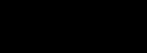
\includegraphics[width=0.6\textwidth]{assets/junit.pdf}
		\caption{Logo of JUnit 5}
	\end{minipage}
\end{figure}
% !TeX root = ../../thesis.tex

\subsection{Maven Surefire}
A commonly used alternative to Gradle is Apache Maven\footnote{\url{http://maven.apache.org/}}. This framework also supports executing JUnit test cases using the Surefire plugin. As opposed to Gradle, Surefire does offer multiple options to specify the order in which the test cases will be executed using the \texttt{runOrder} property. Without any configuration, Maven will run the test cases in alphabetical order. By switching the \texttt{runOrder} property to \texttt{failedFirst}, we can tell Maven to prioritise the previously failed test cases. Another supported value is \texttt{balanced}, which orders test cases based on their duration. Finally, we can choose to implement a custom ordering scheme for absolute control.
% !TeX root = ../../thesis.tex

\subsection{OpenClover}
OpenClover\footnote{\url{https://openclover.org}} is a code coverage tool for Java and Groovy projects. It was created by Atlassian and open-sourced in 2017. OpenClover profiles itself as ``the most sophisticated code coverage tool'', by extracting useful metrics from the coverage results and by providing features that can optimise the test suite. These features include powerful integrations with development software and prominent Continuous Integration systems. Furthermore, OpenClover can automatically analyse the coverage results to detect relations between the application source code and the test cases. This feature allows OpenClover to predict which test cases will have been affected, given a set of modifications to the source code. Subsequently, we can interpret these predictions to implement \tcs{} and therefore reduce the test suite execution time.